\documentclass[a4paper, 12pt]{extreport}

\usepackage[T2A]{fontenc}
\usepackage[utf8]{inputenc}
\usepackage[english,russian]{babel}
\usepackage{amssymb,amsfonts,amsmath,mathtext,cite,enumerate,float}
\usepackage{pgfplots}
\usepackage{graphicx}
\usepackage{tocloft}
\usepackage{listings}
\usepackage[table,xcdraw]{xcolor}
\usepackage{caption}
\usepackage{subcaption}
\usepackage{tempora}
\usepackage{adjustbox}
\usepackage{titlesec}
\usepackage{setspace}
\usepackage{geometry}
\usepackage{indentfirst}
\usepackage{pdfpages}
\usepackage{enumerate,letltxmacro}
\usepackage{threeparttable}
\usepackage[hidelinks]{hyperref}
\usepackage{flafter}
\usepackage{enumitem}
\usepackage{multirow}

\usepackage[figure,table]{totalcount}
\usepackage{lastpage}

\setlist{nosep}

\newcommand{\ssr}[1]{\begin{center}
		\LARGE\bfseries{#1}
	\end{center} \addcontentsline{toc}{chapter}{#1}  }

\makeatletter
\renewcommand\LARGE{\@setfontsize\LARGE{22pt}{20}}
\renewcommand\Large{\@setfontsize\Large{20pt}{20}}
\renewcommand\large{\@setfontsize\large{16pt}{20}}
\makeatother
\RequirePackage{titlesec}
\titleformat{\chapter}[block]{\hspace{\parindent}\large\bfseries}{\thechapter}{0.5em}{\large\bfseries\raggedright}
\titleformat{name=\chapter,numberless}[block]{\hspace{\parindent}}{}{0pt}{\large\bfseries\centering}
\titleformat{\section}[block]{\hspace{\parindent}\large\bfseries}{\thesection}{0.5em}{\large\bfseries\raggedright}
\titleformat{\subsection}[block]{\hspace{\parindent}\large\bfseries}{\thesubsection}{0.5em}{\large\bfseries\raggedright}
\titleformat{\subsubsection}[block]{\hspace{\parindent}\large\bfseries}{\thesubsection}{0.5em}{\large\bfseries\raggedright}
\titlespacing{\chapter}{12.5mm}{-22pt}{10pt}
\titlespacing{\section}{12.5mm}{10pt}{10pt}
\titlespacing{\subsection}{12.5mm}{10pt}{10pt}
\titlespacing{\subsubsection}{12.5mm}{10pt}{10pt}

\makeatletter
\renewcommand{\@biblabel}[1]{#1.}
\makeatother

\geometry{left=30mm, right=10mm, top=20mm, bottom=20mm}

\onehalfspacing

\renewcommand{\theenumi}{\arabic{enumi}}
\renewcommand{\labelenumi}{\arabic{enumi}\text{)}}
\renewcommand{\theenumii}{.\arabic{enumii}}
\renewcommand{\labelenumii}{\asbuk{enumii}\text{)}}
\renewcommand{\theenumiii}{.\arabic{enumiii}}
\renewcommand{\labelenumiii}{\arabic{enumi}.\arabic{enumii}.\arabic{enumiii}.}

\renewcommand{\cftchapleader}{\cftdotfill{\cftdotsep}}

\addto\captionsrussian{\renewcommand{\figurename}{Рисунок}}
\DeclareCaptionLabelSeparator{dash}{~---~}
\captionsetup{labelsep=dash}

\captionsetup[figure]{justification=centering,labelsep=dash}
\captionsetup[table]{labelsep=dash,justification=raggedright,singlelinecheck=off}

\graphicspath{{images/}}

\newcommand{\floor}[1]{\lfloor #1 \rfloor}

\lstset{ %
	language=caml,                 
	basicstyle=\small\ttfamily, 
	numbers=none,               
	showspaces=false,            
	showstringspaces=false,      
	showtabs=false,             
	frame=single,              
	tabsize=2,                 
	captionpos=t,              
	breaklines=true,           
	breakatwhitespace=false, 
	escapeinside={\#*}{*)},   
	abovecaptionskip=-5pt
}

\pgfplotsset{width=0.85\linewidth, height=0.5\columnwidth}

\linespread{1.3}

\parindent=1.25cm

\def\labelitemi{---}
\setlist[itemize]{leftmargin=1.25cm, itemindent=0.65cm}
\setlist[enumerate]{leftmargin=1.25cm, itemindent=0.55cm}

\newcommand{\specialcell}[2][c]{%
	\begin{tabular}[#1]{@{}c@{}}#2\end{tabular}}

\frenchspacing

\begin{document}

% Титульная страница без нумерации
\begin{titlepage}
	\newgeometry{pdftex, left=2cm, right=2cm, top=2.5cm, bottom=2.5cm}
	\fontsize{12pt}{12pt}\selectfont
	\noindent \begin{minipage}{0.15\textwidth}
		
\includegraphics[width=\linewidth]{img/b_logo.png}
	\end{minipage}
	\noindent\begin{minipage}{0.9\textwidth}\centering
		\textbf{Министерство науки и высшего образования Российской Федерации}\\
		\textbf{Федеральное государственное бюджетное образовательное учреждение высшего образования}\\
		\textbf{«Московский государственный технический университет имени Н. Э.~Баумана}\\
		\textbf{(национальный исследовательский университет)»}\\
		\textbf{(МГТУ им. Н. Э.~Баумана)}
	\end{minipage}

	\noindent\rule{18cm}{3pt}
	\newline\newline
	\noindent ФАКУЛЬТЕТ $\underline{\text{«Информатика и системы управления»~~~~~~~~~~~~~~~~~~~~~~~~~~~~~~~~~~~~~~~~~~~~~~~~~~~~~~~}}$ \newline\newline
	\noindent КАФЕДРА $\underline{\text{«Программное обеспечение ЭВМ и информационные технологии»~~~~~~~~~~~~~~~~~~~~~~~}}$\newline\newline\newline\newline\newline\newline\newline

	\begin{center}
		\noindent\begin{minipage}{1.3\textwidth}\centering
		\Large\textbf{   ~~~ Лабораторная работа №3}\newline
		\textbf{по дисциплине <<Анализ Алгоритмов>>}\newline\newline\newline
		\end{minipage}
	\end{center}

	\noindent\textbf{Тема} 			$\underline{\text{Поиск в словаре}}$\newline\newline
	\noindent\textbf{Студент} 		$\underline{\text{Платонова М. И.}}$\newline\newline
	\noindent\textbf{Группа} 		$\underline{\text{ИУ7-51Б}}$\newline\newline
	\noindent\textbf{Преподаватель} $\underline{\text{Волкова Л. Л.}}$\newline

	\begin{center}
		\vfill
		Москва~---~\the\year
		~г.
	\end{center}
	\restoregeometry
\end{titlepage}

\pagenumbering{arabic}
\setcounter{page}{2}

\def\contentsname{\begin{center}\MakeUppercase{СОДЕРЖАНИЕ}\end{center}}
\tableofcontents



\chapter*{ВВЕДЕНИЕ}
\addcontentsline{toc}{chapter}{ВВЕДЕНИЕ}
В данной лабораторной работе рассматриваются два метода поиска элементов в массиве: поиск полным перебором и бинарный поиск. Линейный поиск выполняется путём последовательного сравнения каждого элемента массива с искомым значением, пока оно не будет обнаружено или не завершится обход всех элементов. Бинарный поиск ускоряет этот процесс, сокращая область поиска в два раза на каждом шаге, начиная с проверки среднего элемента оставшегося диапазона, но требует заранее отсортированного массива.

Алгоритмы поиска имеют важное значение в программировании, так как массивы применяются во многих сферах, включая компьютерную графику, анализ данных и машинное обучение. Повышение эффективности поиска позволяет значительно уменьшить время обработки данных, улучшая производительность программ и облегчая работу разработчика.

Целью данной лабораторной работы является исследование двух алгоритмов поиска элемента в массиве: бинарного и линейного (полным перебором).

Для достижения этой цели необходимо выполнить следующие задачи:
\begin{itemize}
    \item[--] рассмотреть и реализовать алгоритм линейного поиска элемента в массиве;
    \item[--] рассмотреть и реализовать алгоритм бинарного поиска элемента в массиве;
    \item[--] провести исследование зависимости количества сравнений от позиции искомого элемента в массиве;
    \item[--] подготовить графики, отображающие результаты сравнительного анализа;
    \item[--] разработать набор тестов для оценки работоспособности реализованных алгоритмов;
    \item[--] сформулировать и представить результаты в отчёте о проведённой лабораторной работе.
\end{itemize}

\chapter{Аналитическая часть}
В этом разделе рассматриваются два метода поиска элементов в массиве: поиск полным перебором и бинарный поиск~\cite{bib1}.

\section{Алгоритмы поиска элементов в массиве}

\subsection{Поиск полным перебором}
Поиск полным перебором -- один из простейших алгоритмов для нахождения элемента в массиве. Он предполагает последовательное сравнение каждого элемента массива с искомым значением, начиная с первого элемента и до тех пор, пока либо не будет найдено совпадение, либо не будут проверены все элементы массива.

Пусть задан массив длины $n$. Сложность алгоритма для такого массива оценивается как $O(n)$. Линейный поиск не требует дополнительных структур данных или сортировки массива и занимает минимальное количество памяти. В каждой итерации цикла алгоритма выполняются операции индексации и сравнения. Для данного алгоритма выделяют один лучший и два худших случая по количеству операций:

\begin{equation}
    \label{eq:search_case}
    f = 
    \begin{cases}
      1, & \text{если элемент находится на первой позиции} \\ 
      n, & \text{иначе, если элемент не найден или найден на последнем сравнении}
    \end{cases}
\end{equation}

Пусть на старте алгоритм поиска выполняется $k_0$ операций, и при каждом сравнении требуется ещё $k_1$ операций (где $k_0$ и $k_1$ -- константы). Тогда количество операций можно выразить следующим образом:

\begin{itemize}
    \item[--] В лучшем случае, когда элемент находится на первой позиции: $k_0 + k_1$
    \item[--] Если элемент найден на второй позиции: $k_0 + 2 \cdot k_1$
    \item В случае, если элемент найден на последней позиции: $k_0 + n \cdot k_1$
    \item[--] Если элемент не найден совсем $k_0 + n \cdot k_1$
\end{itemize}

\subsection{Бинарный поиск}
Бинарный поиск является более оптимизированным методом для поиска в отсортированном массиве, поскольку он сокращает количество элементов для проверки на каждой итерации, что ускоряет процесс.

Алгоритм бинарного поиска делит массив на две части на каждом шаге, проверяя, совпадает ли искомый элемент со значением в середине текущего диапазона. Если значение не совпадает, то в зависимости от результата сравнения выбирается либо левая, либо правая половина массива для следующей проверки. Этот процесс продолжается, пока не будет найден элемент или пока массив не будет исчерпан.

Пусть массив имеет длину $n$. Сложность алгоритма бинарного поиска оценивается как $O(\log n)$, поскольку количество проверок уменьшается на каждом шаге вдвое. Для бинарного поиска, как и для линейного, выделяются один лучший и два худших случая:

\begin{equation}
    \label{eq:search_case_average}
    f = 
    \begin{cases}
      1, & \text{если элемент находится в середине массива} \\ 
      \log_2(n), & \text{иначе, если элемент отсутствует или найден на последней проверке}
    \end{cases} 
\end{equation}

Если элемент находится в середине массива, его можно найти за одну операцию. Если же элемент отсутствует или находится в краю массива, нам нужно будет пройти через все уровни бинарного деления, чтобы проверить последний элемент.
Бинарный поиск требует, чтобы массив был отсортирован перед началом поиска, но не требует дополнительных структур данных. Это делает его эффективным для больших объёмов данных, где линейный поиск становится непрактичным.

\section*{Вывод}
В данном разделе рассмотрены алгоритмы полным перебором и бинарного поиска. Линейный поиск удобен для неупорядоченных массивов, но его сложность $O(\log n)$ ограничивает эффективность при больших объёмах данных. Бинарный поиск, обладающий сложностью $O(\log_2 n)$, работает гораздо быстрее на отсортированных массивах, что делает его подходящим для работы с большими данными, несмотря на необходимость предварительной сортировки.

\chapter{Конструкторская часть}

В данном разделе представлены описания алгоритмов поиска элемента в массиве, а также структуры программного обеспечения и оценки трудоёмкости для каждого метода.

\section{Описание структуры ПО}

На вход программного продукта передан массив $arr$, состоящий из целых чисел, и случайное значение, которое необходимо найти. Программа позволяет пользователю выбрать один из двух алгоритмов поиска: поиск полным перебором или бинарный поиск. В случае бинарного поиска массив предварительно сортируется.

\section{Описание алгоритмов}

В программном продукте реализованы два алгоритма поиска:
\begin{enumerate}
    \item[--] Линейный поиск, выполняющий последовательный перебор элементов массива для нахождения заданного значения.
    \item[--] Бинарный поиск, который применяется к предварительно отсортированному массиву и позволяет эффективно находить элемент.
\end{enumerate}

Для сортировки массива перед выполнением бинарного поиска используется алгоритм сортировки слиянием. Алгоритм сортировки слиянием делит массив на части, которые сортируются и объединяются, обеспечивая упорядоченность элементов массива.

\section{Алгоритм взаимодействия с пользователем}

Программа взаимодействует с пользователем через консоль:
\begin{itemize}
    \item[--] Пользователь вводит номер индивидуальной задачи, который влияет на параметры генерации массива;
    \item[--] Генерируется массив заданной длины из случайных целых чисел;
    \item[--] Программа выполняет линейный поиск случайного элемента и выводит его позицию и время выполнения;
    \item[--] Массив сортируется с помощью алгоритма сортировки слиянием;
    \item[--] Выполняется бинарный поиск первого элемента отсортированного массива, и выводятся его позиция и время выполнения.
\end{itemize}

На рисунках~\ref{fig:lin} и~\ref{fig:bin} представлены схемы реализованных алгоритмов линейного и бинарного поиска.
\clearpage

\begin{figure}[H]
    \centering
    \makebox[\textwidth][c]{\adjustbox{scale=0.5, center, right=20cm}{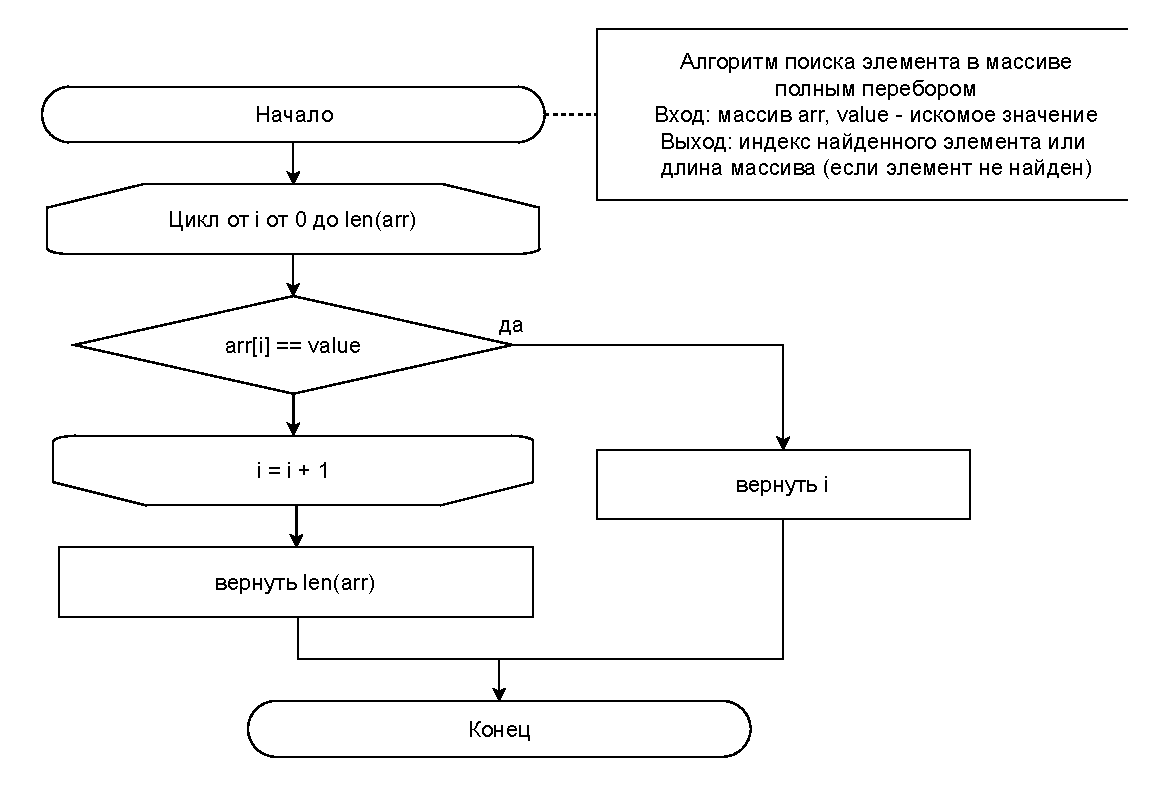
\includegraphics{img/lin.pdf}}}
    \caption{Алгоритм поиска элемента в массиве полным перебором}
    \label{fig:lin}
\end{figure}

\begin{figure}[H]
    \centering
    \adjustbox{scale=0.6, center}{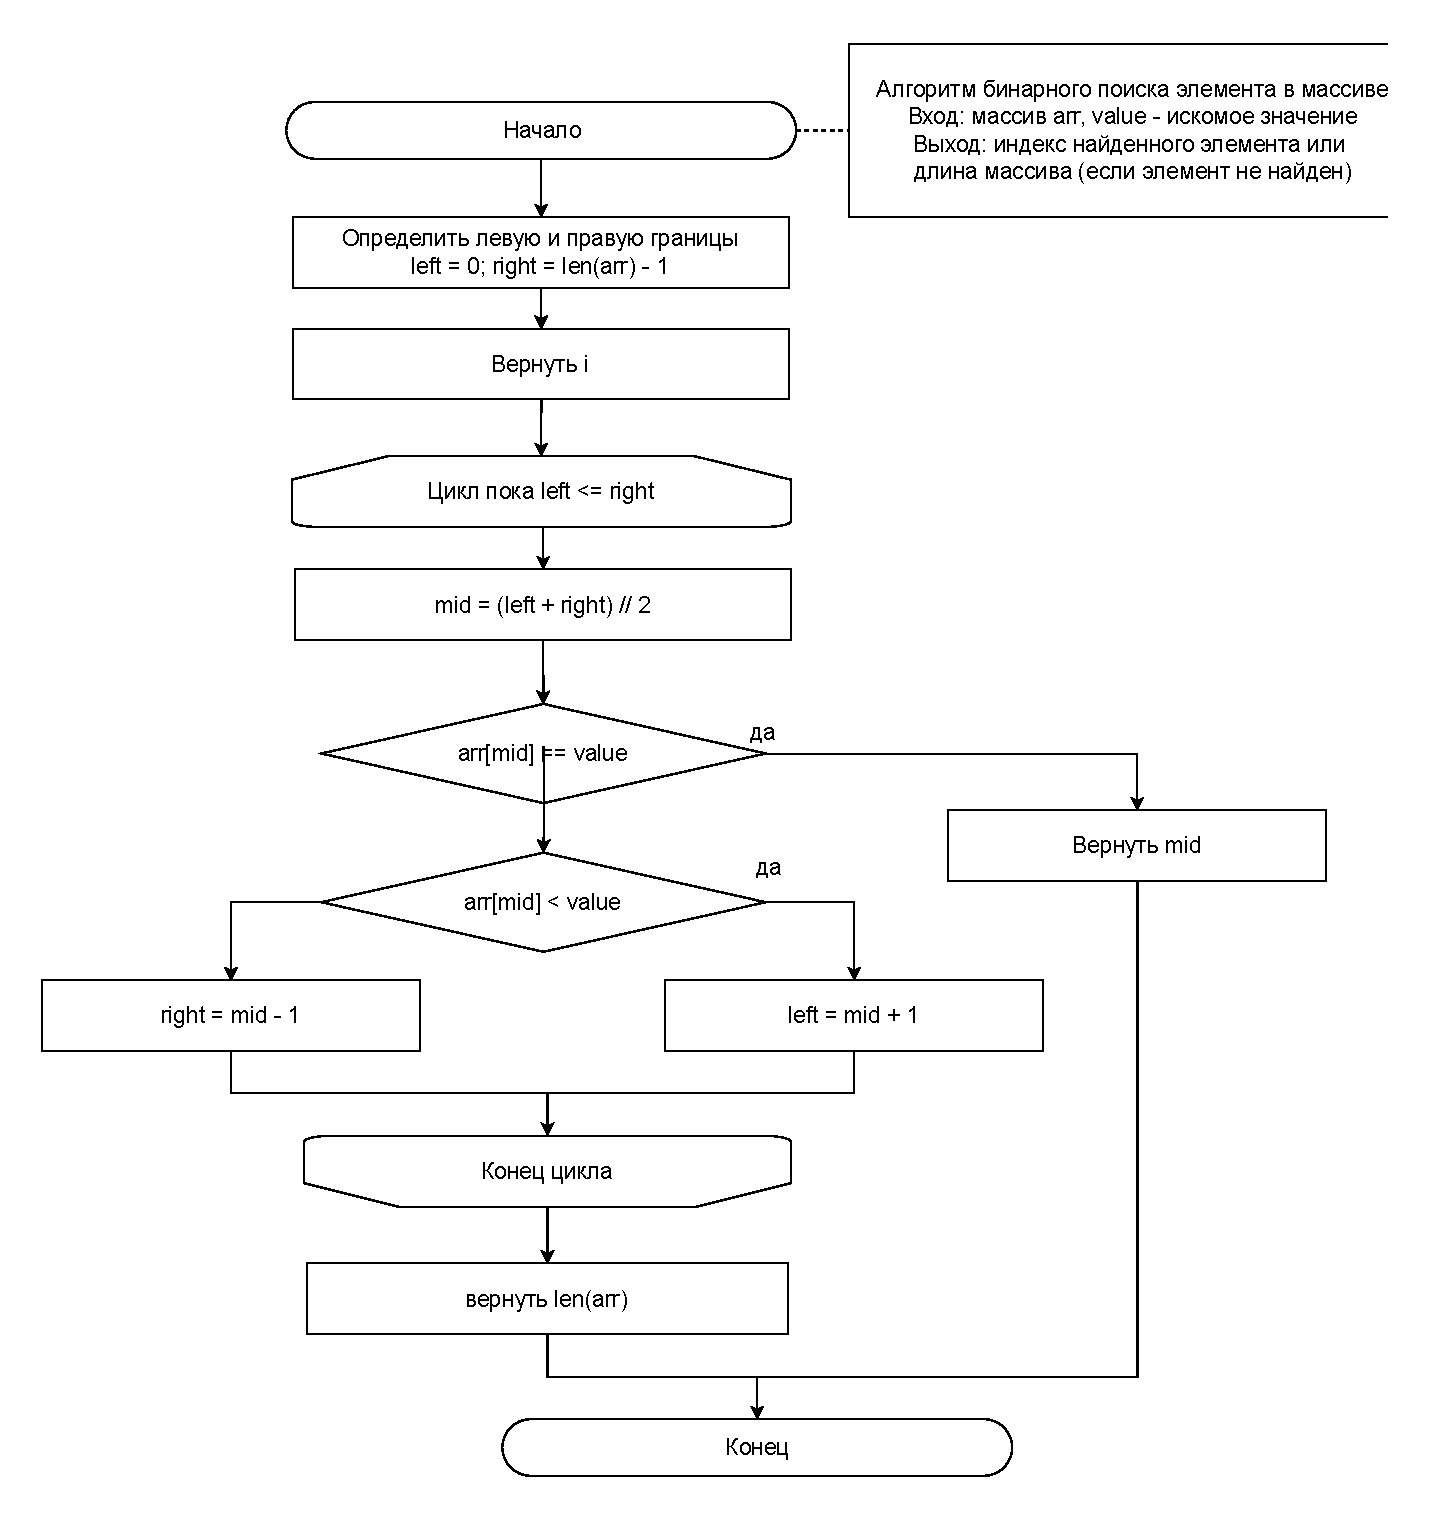
\includegraphics{img/bin.pdf}}
    \caption{Алгоритм бинарного поиска элемента в массиве}
    \label{fig:bin}
\end{figure}

\clearpage

\chapter{Технологическая часть}
В данном разделе приведены данные о выбранном языке программирования, реализации алгоритмов поиска и тестировании каждого алгоритма.

\section{Требования к программному обеспечению}
\begin{itemize}
    \item[--] Входные данные: массив \texttt{arr}, состоящий из целых чисел, и значение, которое необходимо найти в этом массиве.
    \item[--] Выходные данные: индекс найденного элемента в массиве или, если элемент не найден, длина массива (что указывает на отсутствие значения).
\end{itemize}

\section{Средства реализации}
Для реализации алгоритмов поиска, проведения замеров времени и обработки данных в данной работе используется язык программирования \texttt{Python}~\cite{bib3}. \texttt{Python} предоставляет все необходимые инструменты для работы с массивами и измерения времени выполнения. 

Для разработки алгоритмов используются следующие типы и структуры данных:
\begin{itemize}
    \item[--] Одномерный массив целых чисел \texttt{arr}, в котором выполняется поиск.
    \item[--] Переменные для хранения текущих индексов и границ поиска.
\end{itemize}

Замеры времени выполняются с помощью функции \textit{time}~\cite{bib4}.

\section{Структура программы}
Программа состоит из нескольких модулей: 
\begin{itemize}
    \item[--] \texttt{algs.py} -- файл, содержащий реализацию всех алгоритмов; 
    \item[--] \texttt{compare.py} -- модуль для сравнения времени выполнения алгоритмов поиска.
\end{itemize}

\section{Описание работы программы}
Программа взаимодействует с пользователем через консоль:
\begin{itemize}
    \item[--] Пользователь вводит номер индивидуальной задачи, что влияет на генерацию параметров массива.
    \item[--] Генерируется массив случайных чисел заданной длины и диапазона.
    \item[--] Выполняется линейный поиск случайного значения в массиве и выводится его позиция и время выполнения.
    \item[--] Массив сортируется с использованием сортировки слиянием для подготовки к бинарному поиску.
    \item[--] Выполняется бинарный поиск первого элемента отсортированного массива, выводятся его позиция и время выполнения.
\end{itemize}


\section{Реализация алгоритмов}
В листинге~\ref{lst:calculate_length} представлена реализация функции \texttt{calculate\_length}, которая вычисляет длину на основе заданного числа \( X \).

\begin{center}
\captionsetup{justification=raggedright,singlelinecheck=off}
\begin{lstlisting}
def calculate_length(X):
    if X // 8 + (X >> 2) % 10 == 0:
        return X % 1000
    else:
        return ((X >> 2) % 10 * (X % 10) + (X >> 1) % 10)
\end{lstlisting}
\captionsetup{justification=centering, singlelinecheck=off}
\captionof{lstlisting}{Реализация функции расчёта длины на основе номера задачи}
\label{lst:calculate_length}
\end{center}

В листинге~\ref{lst:normal_search} представлена реализация функции \texttt{normal\_search}, которая осуществляет линейный поиск элемента в массиве.

\begin{center}
\captionsetup{justification=raggedright,singlelinecheck=off}
\begin{lstlisting}
def normal_search(arr, value):
    for i in range(len(arr)):
        if arr[i] == value:
            return i
    return len(arr) 
\end{lstlisting}
\captionsetup{justification=centering, singlelinecheck=off}
\captionof{lstlisting}{Реализация линейного поиска элемента в массиве}
\label{lst:normal_search}
\end{center}

В листинге~\ref{lst:binary_search} представлена реализация функции \texttt{binary\_search}, которая выполняет бинарный поиск элемента в отсортированном массиве.

\begin{center}
\captionsetup{justification=raggedright,singlelinecheck=off}
\begin{lstlisting}
def binary_search(arr, value):
    left, right = 0, len(arr) - 1
    while left <= right:
        mid = (left + right) // 2
        if arr[mid] == value:
            return mid
        elif arr[mid] < value:
            left = mid + 1
        else:
            right = mid - 1
    return len(arr)  
\end{lstlisting}
\captionsetup{justification=centering, singlelinecheck=off}
\captionof{lstlisting}{Реализация бинарного поиска элемента в отсортированном массиве}
\label{lst:binary_search}
\end{center}

В листинге~\ref{lst:merge} представлена реализация функции \texttt{merge}, которая объединяет две части массива во время выполнения сортировки слиянием.

\begin{center}
\captionsetup{justification=raggedright,singlelinecheck=off}
\begin{lstlisting}
def merge(arr, left, mid, right):
    n1 = mid - left + 1
    n2 = right - mid
    left_part = arr[left:left + n1]
    right_part = arr[mid + 1:mid + 1 + n2]
    
    i = j = 0
    result = []
    while i < n1 and j < n2:
        if left_part[i] <= right_part[j]:
            result.append(left_part[i])
            i += 1
        else:
            result.append(right_part[j])
            j += 1

    result.extend(left_part[i:])
    result.extend(right_part[j:])
    
    for k in range(n1 + n2):
        arr[left + k] = result[k]
\end{lstlisting}
\captionsetup{justification=centering, singlelinecheck=off}
\captionof{lstlisting}{Реализация функции слияния для сортировки}
\label{lst:merge}
\end{center}

В листинге~\ref{lst:merge_sort} представлена реализация функции \texttt{merge\_sort}, которая сортирует массив с помощью алгоритма сортировки слиянием.

\begin{center}
\captionsetup{justification=raggedright,singlelinecheck=off}
\begin{lstlisting}
def merge_sort(arr, left, right):
    if left < right:
        mid = (left + right) // 2
        merge_sort(arr, left, mid)
        merge_sort(arr, mid + 1, right)
        merge(arr, left, mid, right)
\end{lstlisting}
\captionsetup{justification=centering, singlelinecheck=off}
\captionof{lstlisting}{Реализация сортировки слиянием}
\label{lst:merge_sort}
\end{center}

\clearpage


\section{Функциональные тесты}
В таблицах~\ref{tbl:functional_test_binary_search} и~\ref{tbl:functional_test_full_search} приведены функциональные тесты для алгоритмов бинарного поиска и полного перебора элементов в массиве. Все тесты выполнены успешно, фактические результаты совпадают с ожидаемыми.
\begin{table}[h]
    \centering
    \captionsetup{justification=centering}
    \resizebox{\textwidth}{!}{%
        \begin{tabular}{|r|r|r|r|r|}
            \hline
            \textbf{Размер массива} & \textbf{Массив} & \textbf{Элемент поиска} & \textbf{Бинарный поиск} & \textbf{Ожидаемый результат} \\
            \hline
            0 & [] & 0 & не найден, кол-во сравн. 0 & не найден, кол-во сравн. 0 \\
            \hline
            1 & [0] & 0 & индекс 0, кол-во сравн. 1 & индекс 0, кол-во сравн. 1 \\
            \hline
            1 & [0] & 1 & не найден, кол-во сравн. 1 & не найден, кол-во сравн. 1 \\
            \hline
            2 & [0, 1] & 0 & индекс 0, кол-во сравн. 1 & индекс 0, кол-во сравн. 1 \\
            \hline
            2 & [0, 1] & 1 & индекс 1, кол-во сравн. 2 & индекс 1, кол-во сравн. 2 \\
            \hline
            4 & [1, 2, 3, 4] & 3 & индекс 2, кол-во сравн. 2 & индекс 2, кол-во сравн. 2 \\
            \hline
            8 & [1, 3, 5, 7, 9, 11, 13, 15] & 9 & индекс 4, кол-во сравн. 3 & индекс 4, кол-во сравн. 3 \\
            \hline
            8 & [1, 3, 5, 7, 9, 11, 13, 15] & 16 & не найден, кол-во сравн. 4 & не найден, кол-во сравн. 4 \\
            \hline
        \end{tabular}%
    }
    \caption{Функциональные тесты для бинарного поиска элемента в массиве}
    \label{tbl:functional_test_binary_search}
\end{table}

\begin{table}[h]
    \centering
    \captionsetup{justification=centering}
    \resizebox{\textwidth}{!}{%
        \begin{tabular}{|r|r|r|r|r|}
            \hline
            \textbf{Размер массива} & \textbf{Массив} & \textbf{Элемент поиска} & \textbf{Полный перебор} & \textbf{Ожидаемый результат} \\
            \hline
            0 & [] & 0 & не найден, кол-во сравн. 0 & не найден, кол-во сравн. 0 \\
            \hline
            1 & [0] & 0 & индекс 0, кол-во сравн. 1 & индекс 0, кол-во сравн. 1 \\
            \hline
            1 & [0] & 1 & не найден, кол-во сравн. 1 & не найден, кол-во сравн. 1 \\
            \hline
            2 & [0, 1] & 0 & индекс 0, кол-во сравн. 1 & индекс 0, кол-во сравн. 1 \\
            \hline
            2 & [0, 1] & 1 & индекс 1, кол-во сравн. 2 & индекс 1, кол-во сравн. 2 \\
            \hline
            4 & [1, 2, 3, 4] & 3 & индекс 2, кол-во сравн. 3 & индекс 2, кол-во сравн. 3 \\
            \hline
            8 & [1, 3, 5, 7, 9, 11, 13, 15] & 9 & индекс 4, кол-во сравн. 5 & индекс 4, кол-во сравн. 5 \\
            \hline
            8 & [1, 3, 5, 7, 9, 11, 13, 15] & 16 & не найден, кол-во сравн. 8 & не найден, кол-во сравн. 8 \\
            \hline
        \end{tabular}%
    }
    \caption{Функциональные тесты для полного перебора элемента в массиве}
    \label{tbl:functional_test_full_search}
\end{table}


\section*{Вывод}
Результаты тестирования подтверждают, что оба алгоритма корректно выполняют поиск: бинарный поиск эффективен для отсортированных массивов, а полный перебор гарантирует нахождение элемента независимо от порядка массива. Все тесты успешно завершены, результаты совпадают с ожидаемыми.
\newpage

\chapter{Исследовательская часть}
В данном разделе представлены результаты исследования эффективности работы алгоритмов по времени выполнения, основанной на критерии временных затрат.

\section{Влияние позиции элемента на количество сравнений в алгоритмах}

Для тестирования алгоритмов использовались данные, представленные в виде словарей, где ключи -- это строки, а значения -- соответствующие хэши. Объём массива вычислялся по следующей формуле:
\begin{equation}
    \label{eq:length}
    \text{length} = 
    \begin{cases} 
      X \% 1000, & \text{если } X \equiv 0 \mod 8 \\ 
      (X >> 2) \% 10 \cdot (X \% 10) + (X >> 1) \% 10, & \text{иначе}
    \end{cases}
\end{equation}

где $X$ -- номер индивидуального задания.

Для проведения замеров выбран массив длиной 1000 элементов, заполненный случайными хэшами. 

\section{Поиск полным перебором}
На рисунке~\ref{fig:linear_search} представлена гистограмма для линейного поиска.
\begin{figure}[htbp] 
    \centering
    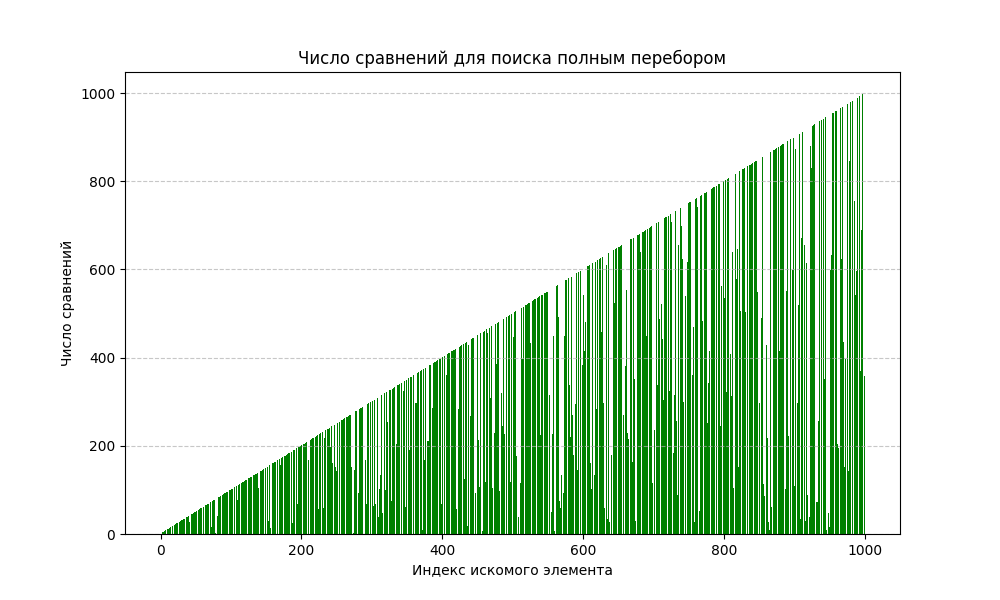
\includegraphics[scale=0.5]{img/lin_search.png}
    \caption{Зависимость количества сравнений от позиции элемента в массиве при линейном поиске.}
    \label{fig:linear_search}
\end{figure}
\newpage


Линейный поиск -- это алгоритм, при котором каждый элемент массива проверяется последовательно до тех пор, пока не будет найден нужный элемент или не завершится обход всего массива. Этот метод имеет сложность $(O(n)$, так как в худшем случае требуется пройти весь массив.

Выполненные замеры демонстрируют, что количество сравнений в линейном поиске зависит от позиции элемента: чем ближе элемент к началу массива, тем меньше сравнений требуется для его нахождения. В случае отсутствия искомого элемента линейный поиск выполняет наибольшее количество сравнений, равное длине массива. 

\section{Бинарный поиск}
На рисунке~\ref{fig:binary_search} представлена гистограмма для бинарного поиска.
\begin{figure}[htbp]  
    \centering
    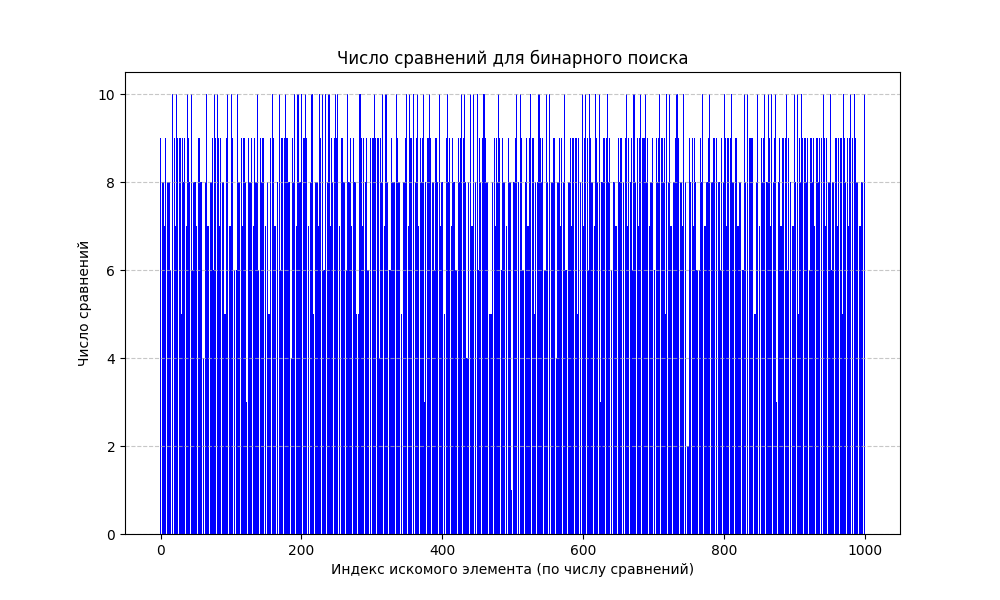
\includegraphics[scale=0.5]{img/bin_search.png}
    \caption{Зависимость количества сравнений от позиции элемента в массиве при бинарном поиске.}
    \label{fig:binary_search}
\end{figure}
\newpage
На рисунке~\ref{fig:count_search} представлена гистограмма, отображающая результаты для бинарного поиска.
\begin{figure}[htbp]  
    \centering
    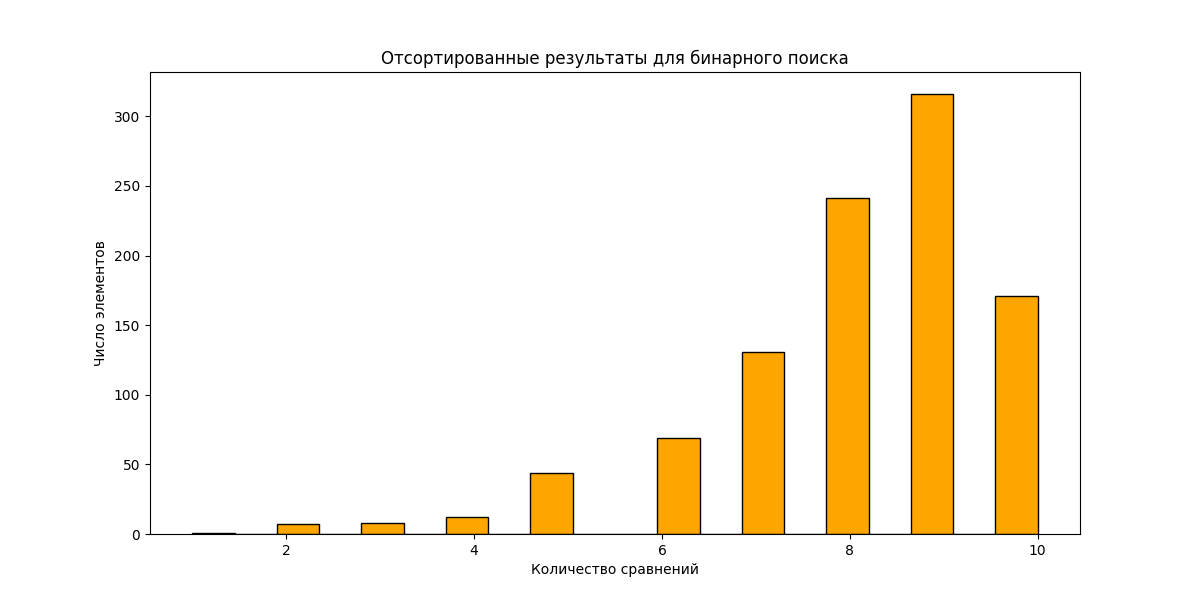
\includegraphics[scale=0.5]{img/4.png}
    \caption{Результаты для бинарного алгоритма.}
    \label{fig:count_search}
\end{figure}

Бинарный поиск требует предварительной сортировки массива и использует метод деления пополам для поиска элемента. Сложность этого алгоритма равна $O(\log n)$, что позволяет значительно сократить количество сравнений по сравнению с линейным поиском. Однако для выполнения бинарного поиска массив должен быть отсортированным, что может добавить к общей сложности.

При выполнении бинарного поиска для большинства элементов требуется от 8 до 10 сравнений, что делает его гораздо более быстрым по сравнению с полным перебором, где может потребоваться гораздо больше шагов для нахождения элемента.

\section*{Вывод}
Линейный поиск требует большее количество сравнений по сравнению с бинарным поиском, особенно при увеличении размера массива. В случаях, когда массив уже отсортирован, бинарный поиск является более эффективным методом. Линейный поиск остаётся удобным для неупорядоченных массивов, но при больших объёмах данных бинарный поиск позволяет достичь более высокой скорости за счёт уменьшения количества сравнений.

\chapter*{ЗАКЛЮЧЕНИЕ}
\addcontentsline{toc}{chapter}{ЗАКЛЮЧЕНИЕ}
Цель работы достигнута. В ходе выполнения данной лабораторной работы решены следующие задачи:
\begin{itemize}
    \item[--] рассмотрен и реализован алгоритм линейного поиска элемента в массиве;
    \item[--] рассмотрен и реализован алгоритм бинарного поиска элемента в массиве;
    \item[--] проведено исследование зависимости количества сравнений от позиции искомого элемента в массиве, что позволило выявить особенности работы каждого алгоритма;
    \item[--] подготовлены графики, демонстрирующие результаты сравнительного анализа эффективности алгоритмов;
    \item[--] разработан набор тестов для оценки правильности и производительности реализованных алгоритмов по критериям временных затрат и количества сравнений;
    \item[--] результаты исследования представлены в виде отчёта о выполненной лабораторной работе.
\end{itemize}
Исследования показали, что эффективность поисковых алгоритмов зависит от позиции элемента. Бинарный поиск требует меньше сравнений, чем линейный.

При линейном поиске число сравнений растёт с позицией элемента, что делает его неэффективным для больших массивов. Бинарный поиск, наоборот, увеличивает трудоёмкость логарифмически, что сокращает количество сравнений.

Хотя бинарный поиск обычно демонстрирует лучшую эффективность по сравнению с линейным, его скорость может уменьшаться, если элемент расположен в начале массива. Также необходимо учитывать, что его эффективность зависит от используемого метода сортировки массива.

\renewcommand{\bibname}{СПИСОК ИСПОЛЬЗОВАННЫХ ИСТОЧНИКОВ}
\begin{thebibliography}{4}
    \bibitem{bib1}
    Сборник задач по теории алгоритмов: учеб.-метод. пособие / В. М. Котов [и др.]. -- Минск: БГУ, 2017. -- 183 с. -- ISBN 978-985-566-412-4.

    \bibitem{bib2}
    Ничушкина, Т. Н., Гуренко, В. В. Разработка алгоритмов простейших программ: Электронное учебное издание. -- М.: МГТУ имени Н. Э. Баумана, 2014. -- 47 с., ил.

    \bibitem{bib3}
    Python Software Foundation. Официальная документация по Python [Электронный ресурс]. -- Режим доступа: \url{https://www.python.org/doc/} (дата обращения: 31.10.2024).

    \bibitem{bib4}
    Python Software Foundation. Модуль time -- Доступ к времени и его преобразования [Электронный ресурс]. -- Режим доступа: \url{https://docs.python.org/3/library/time.html} (дата обращения: 31.10.2024).
\end{thebibliography}


\addcontentsline{toc}{chapter}{СПИСОК ИСПОЛЬЗОВАННЫХ ИСТОЧНИКОВ}

\end{document}